\section{Step 5 - A 3D Function}
\subsection{See the result}
In this section we want to draw a function in 3D.
Our function is a spiral around the $z$-axis.
At some points the functions tangent vectors are displayed.
In order to give you an image what we want to create I present the result of our subject in figure~\ref{STEP_5_1_SCREEN}.
Subfigure~\ref{STEP_5_1_1_SCREEN} shows the spiral function and the coordinate cross invented in the last section.
In order to show the spatial property of the spiral subfigure~\ref{STEP_5_1_2_SCREEN} shows a cylinder with the same radius and orientation as the spiral.
% +++++++++++++++++++++++++++++++++++++++++++++++++++++++++++++++++++++++ 
% +++ Bild: Step 5_1 ++++++++++++++++++++++++++++++++++++++++++++++++++++
% +++++++++++++++++++++++++++++++++++++++++++++++++++++++++++++++++++++++ 
\begin{figure}[htbp]
  \centering
  \subfigure[Screenshot of Step5\_1 without the cylinder]{
    \label{STEP_5_1_1_SCREEN}
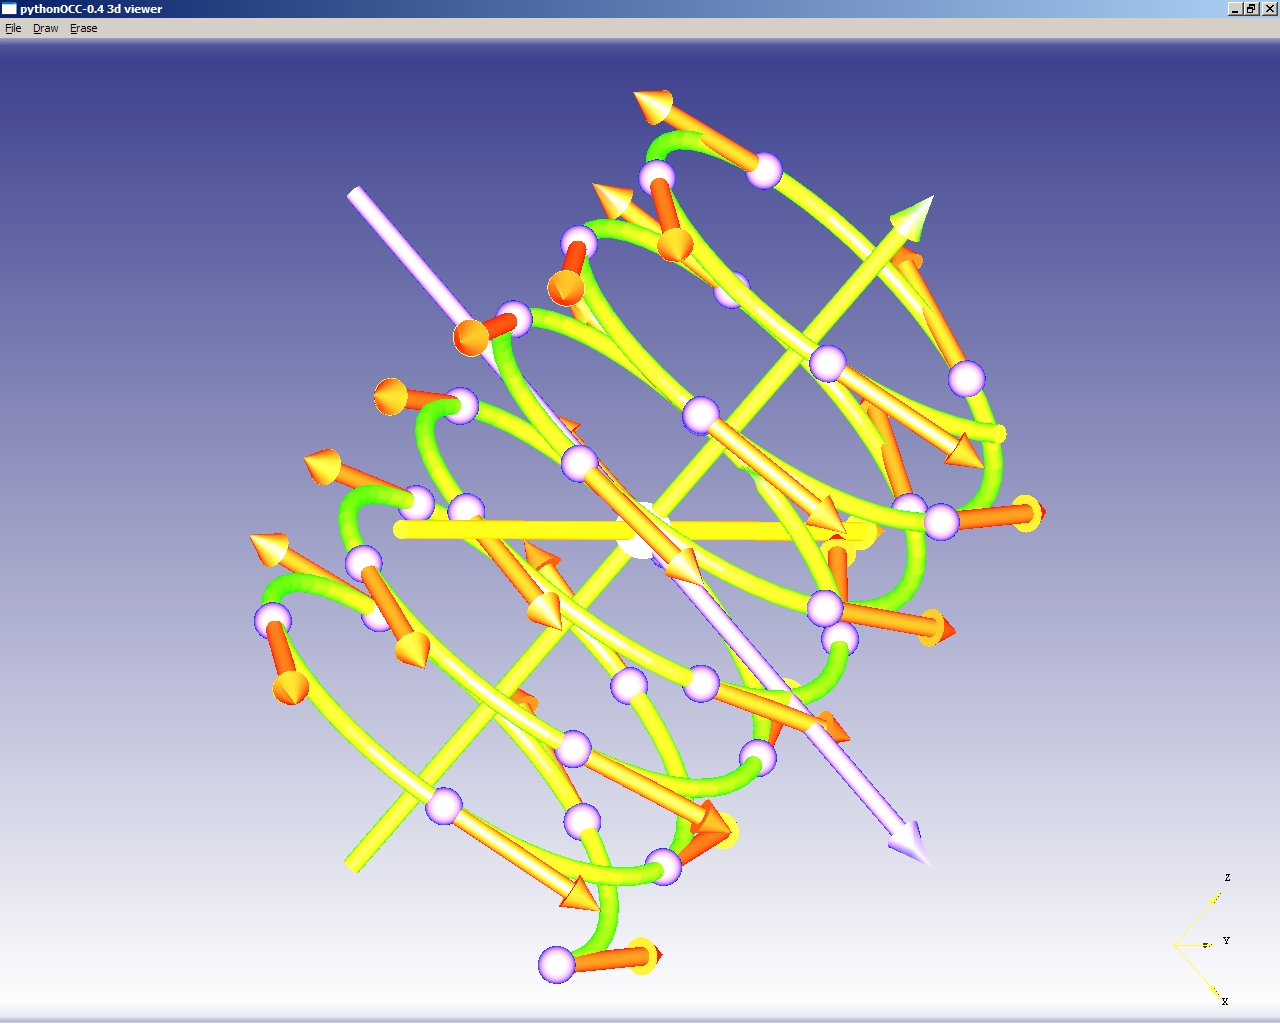
\includegraphics[height=8.5cm,width=11.3cm]{Step5_1_1.jpg}
  }

  \vspace{0.3cm} % Abstand zwischen den subfigures
  \subfigure[Screenshot of Step5\_1 with the cylinder]{
    \label{STEP_5_1_2_SCREEN}
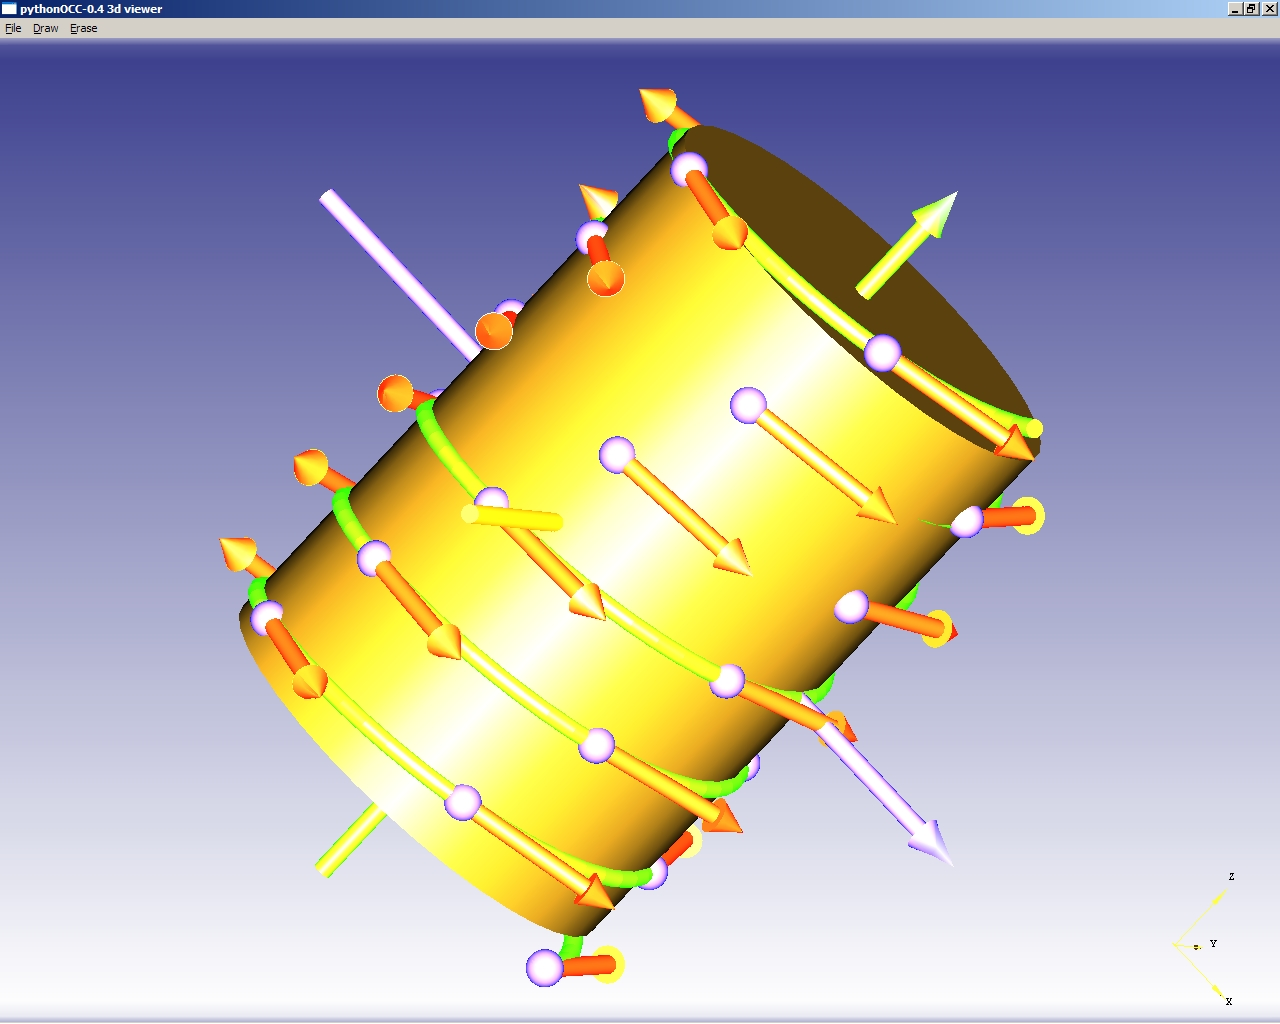
\includegraphics[height=8.5cm,width=11.3cm]{Step5_1_2.jpg}
  }

 \vspace{0.3cm}
  \caption[Screenshots of Step5\_1]{Screenshots of Step5\_1}
  \label{STEP_5_1_SCREEN}
\end{figure}

\subsection{Some formulars}
If you do not know how to construct a spiral and how to compute its tangent vector at a certain point, here is a short presentation of the formulars needed\footnote{It is not my aim to explain maths. Please search on the web or consult a book if you do not understand that. My aim is to give you an example how to draw a fuction in 3D. So if you do not care about math that does not hurt. If you want your functions to be shown take this sample as a template.}.

If you look at a spiral from the top you see a circle if you do not take the perspective into account.
Hence it is no suprise that if we want to create a spiral around the $z$-direction the $x$- and $y$-components of the function create a circle.
Due to the spiral should be regular the $z$-component is a linear function.
So we can write down the formular for our spiral to
\begin{equation}
\label{EQSPIRAL}
\mathbf{C}(t) =
\left( 
\begin{array}{c}
r \, \cos(t) \\
r \, \sin(t) \\
m \, t
\end{array}
\right) \;\;\; .
\end{equation} 
The tangent of that function is the derivative of equation~\ref{EQSPIRAL} with respect to $t$
\begin{equation}
\label{EQTANGSPIRAL}
\frac{\partial\mathbf{C}(t)}{\partial t} =
\left( 
\begin{array}{c}
(-1) \, r \, \sin(t) \\
r \, \cos(t) \\
m 
\end{array}
\right) \;\;\; .
\end{equation} 
